\documentclass[12pt,a4paper]{report}
\usepackage[utf8]{inputenc}
\usepackage[portuguese]{babel}
\usepackage{amsmath}
\usepackage{graphicx}
\usepackage{amsfonts}
\usepackage{amssymb}
\renewcommand{\familydefault}{\sfdefault} %%Muda a fonte para sans-serif
\author{Grupo 5 \\fc51033 Jorge Martins \\ fc51088 Pedro Silva \\ fc51101 Lívio Rodrigues}
\date{}

\usepackage{titlesec}

\titleformat{\chapter}{\normalfont\huge}{\thechapter.}{20pt}{\huge\it}
\begin{document}
\title{Relatório - Raft}
\maketitle
\tableofcontents
\chapter{Principais Componentes}
\section{Cliente}
\subsection{Client}
Classe Cliente que envia em loop infinito requests ao chamar o método request() da classe ClientRaft.
\subsection{ClientRaft}
Classe responsável por se conectar ao líder dos Servidores. Primeiro tenta conectar-se a um servidor aleatório e se esse não for o Leader, ser-lhe-ão enviados os dados do Leader(endereço ip e porto) e de seguida conecta-se ao Leader. Depois de conectado ao Leader, recebe o seu clientID(único) gerado pelo Servidor. \\
Esta Classe vai ainda ser responsável por gerar os IDs das operações(incrementa o id a cada operação realizada).
\subsection{Command}
Classe auxiliar usada para enviar toda a informação para o Líder. Esta Classe contem a string referente ao request enviado pelo Client, o ID do Client em questão e o ID da operação.

\section{Servidor}
\subsection{Service}
Classe recebe o ID do servidor que queremos iniciar e liga esse servidor através da classe ServerRaft. Nesta fase é necessário que o id dado a esta classe seja válido, i.e, exista no ficheiro "config.properties".
\subsection{ServerRaft}
Classe responsável por aceitar conexões de clientes e servidores, que implementa a lógica do algoritmo Raft. Foi usada uma arquitetura MultiThreading de modo a paralelizar o funcionamento do servidor, como iremos explicar mais à frente.
\subsection{StateMachine}
Classe que executa os comandos depois do seu LogEntry correspondente ser commited. Esta classe tem um HashMap que guarda a ultima operacão realizada para cada cliente para que, caso esta se perca e seja requested novamente, a state machine não tenha de realizar novamente a computação.
\subsection{LogEntry}
Entry que vai ficar guardada no Log. Contém o termo, o seu index no Log, o seu comando, o id do cliente que fez o request e o id da operação.
\subsection{Command}
Classe auxiliar usada para enviar toda a informação para o Líder. Esta Classe contém a String referente ao request enviado pelo Client, o ID do Client em questão e o ID da operação.
\subsection{AppendEntries}
Objeto que vai ser enviado do Leader para os Followers. Contém, o termo atual do Leader, o ID do Leader, o último index no Log, o último termo no Log, a LogEntry referente ao pedido e o último index de commit no Leader.
\subsection{AppendEntryResponse}
Resposta aos AppendEntriesRPC. Esta Classe vai servir como resposta dos Followers para o Leader. Contém apenas o termo atual do follower e se o Append foi realizado com sucesso ou não.
\newpage
\section{Ficheiros de Configuração}
Existem dois ficheiros de configuração, um para os Cliente e outro para os Servidores.
\subsection{No Cliente}
O ficheiro no lado do Cliente contem a informação de todos os servidores disponíveis para conexão. Contem o ID, Ip e porto usado por cada servidor.\\
Exemplo: \\
servers=1-127.0.0.1:40000;2-127.0.0.1:40001;3-127.0.0.1:40002;4-127.0.0.1:40003;
\subsection{No Servidor}
O ficheiro no lado do Servidor contem a informação de todos os servidores disponíveis para conexão. Contem o ID, Ip, o porto usado por cada servidor para comunicar com clientes e o porto para comunicar entre servidores.\\
Exemplo: \\
servers=1-127.0.0.1:40000:50000;2-127.0.0.1:40001:50001;3-127.0.0.1:40002:50002;
\chapter{Decisões Arquiteturais}
As principais classes envolvidas na nossa implementação estão representadas no esquema seguinte. Existem duas classes (Client e Service) que servem apenas para executar as aplicações. A implementação do RAFT é feita nas classes ClientRaft e ServerRaft. Temos a classe State Machine que executa as operações a pedido do cliente e, por fim, temos também classes que representam objetos relevantes para o algoritmo RAFT, como a LogEntry, a AppendEntry e a AppendEntryResponse.  
\begin{figure}[h]
\centering
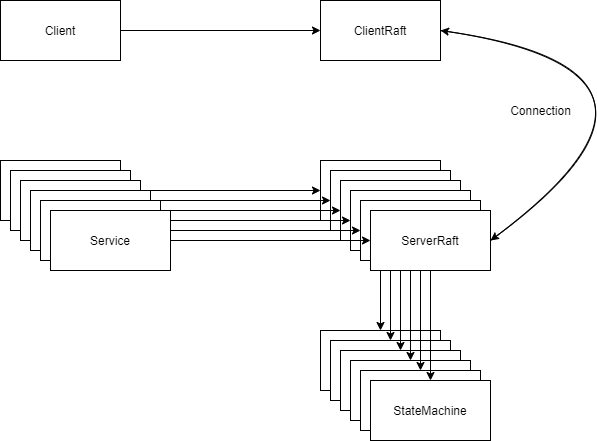
\includegraphics[scale=0.5]{Arquitetura.png} 
\caption{Modelo de Classes}
\end{figure}
\newpage
\section{Arquitetura Multi Thread}
\begin{figure}[h]
\centering
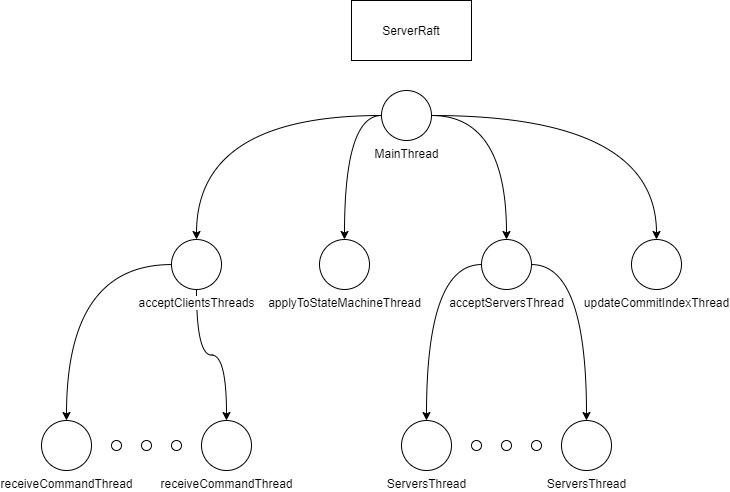
\includegraphics[scale=0.5]{ThreadDiagram.png} 
\caption{Esquema de Threads num Servidor}
\end{figure}
\subsection{Aceitar conexões de clientes}
Implementámos uma thread específica para aceitar conexões de clientes. Uma vez que uma ligação seja aceite é criada uma thread ReceiveCommandsThread para cada cliente aceite.
\subsection{ReceiveCommandsThread}
Esta thread é responsável por receber os pedidos do cliente. Ao receber um pedido cria e adiciona ao Log uma LogEntry referente ao pedido. A thread depois espera que o pedido seja executado para responder ao cliente com o valor computado e guardado na State Machine.
\subsection{Aceitar conexões de servidores}
Para que os servidores sejam capazes de comunicar uns com os outros implementámos uma thread que, à semelhança da thread que aceita conexões de clientes, irá aceitar conexões de outros servidores (de notar que na nossa implementação os servidores apenas se ligam aos servidores que tenham um id superior ao deles, de modo a evitar tentativas de ligação bilaterais). Esta thread irá criar uma thread do tipo ServersThread para cada servidor aceite.
\subsection{ServersThread}
Esta thread terá comportamentos diferentes consoante o servidor onde está a ser executada. Caso seja no Leader ela irá chamar o método "sendRPC" que irá enviar aos followers AppendEntries para cada pedido adicionado ao Log. Caso seja um follower ela irá receber e responder a esses AppendEntries através do método "receiveRPC".
\subsection{Aplicar pedidos à State Machine}
Temos também uma thread que irá verificar constantemente se o commit index do servidor é superior ao lastApplied e, caso o seja, iremos executar o pedido na posição lastApplied do Log.
\subsection{Update ao Commit Index}
Por fim temos uma thread que verifica constantemente os commit index dos followers, através da estrutura de dados "matchIndex". Se o número de servidores que têm um commit index superior ao do Leader for maior que metade dos servidores do cluster, então o commit index do Leader irá ser incrementado.

\chapter{Instruções de Uso}
Para executar o nosso programa foram entregues dois scripts Client.sh e Service.sh nas pastas Client e Server, respetivamente. Deste modo para executar o cliente basta abrir uma consola na pasta Client e correr o comando {\it ./Client.sh}.
Para executar o servidor, é necessário abrir uma consola na pasta Server e correr o comando {\it ./Service.sh $<$serverID$>$}, sendo serverID um dos ids presentes no config.properties.
\\
Também é possível importar a pasta Client e Server como projetos separados no Eclipse e correr normalmente. No entanto deve ser tido em conta que a correr o servidor é necessário colocar o id desejado nos argumentos da run configuration.
\end{document}